\input{"preamble.tex"}

\addbibresource{FourManifolds.bib}

\let\Begin\begin
\let\End\end
\newcommand\wrapenv[1]{#1}

\makeatletter
\def\ScaleWidthIfNeeded{%
 \ifdim\Gin@nat@width>\linewidth
    \linewidth
  \else
    \Gin@nat@width
  \fi
}
\def\ScaleHeightIfNeeded{%
  \ifdim\Gin@nat@height>0.9\textheight
    0.9\textheight
  \else
    \Gin@nat@width
  \fi
}
\makeatother

\setkeys{Gin}{width=\ScaleWidthIfNeeded,height=\ScaleHeightIfNeeded,keepaspectratio}%

\title{
\rule{\linewidth}{1pt} \\
\textbf{
    4-Manifolds
  }
    \\ {\normalsize Lectures by Philip Engel. University of Georgia,
Spring 2021} \\
  \rule{\linewidth}{2pt}
}
\titlehead{
    \begin{center}
  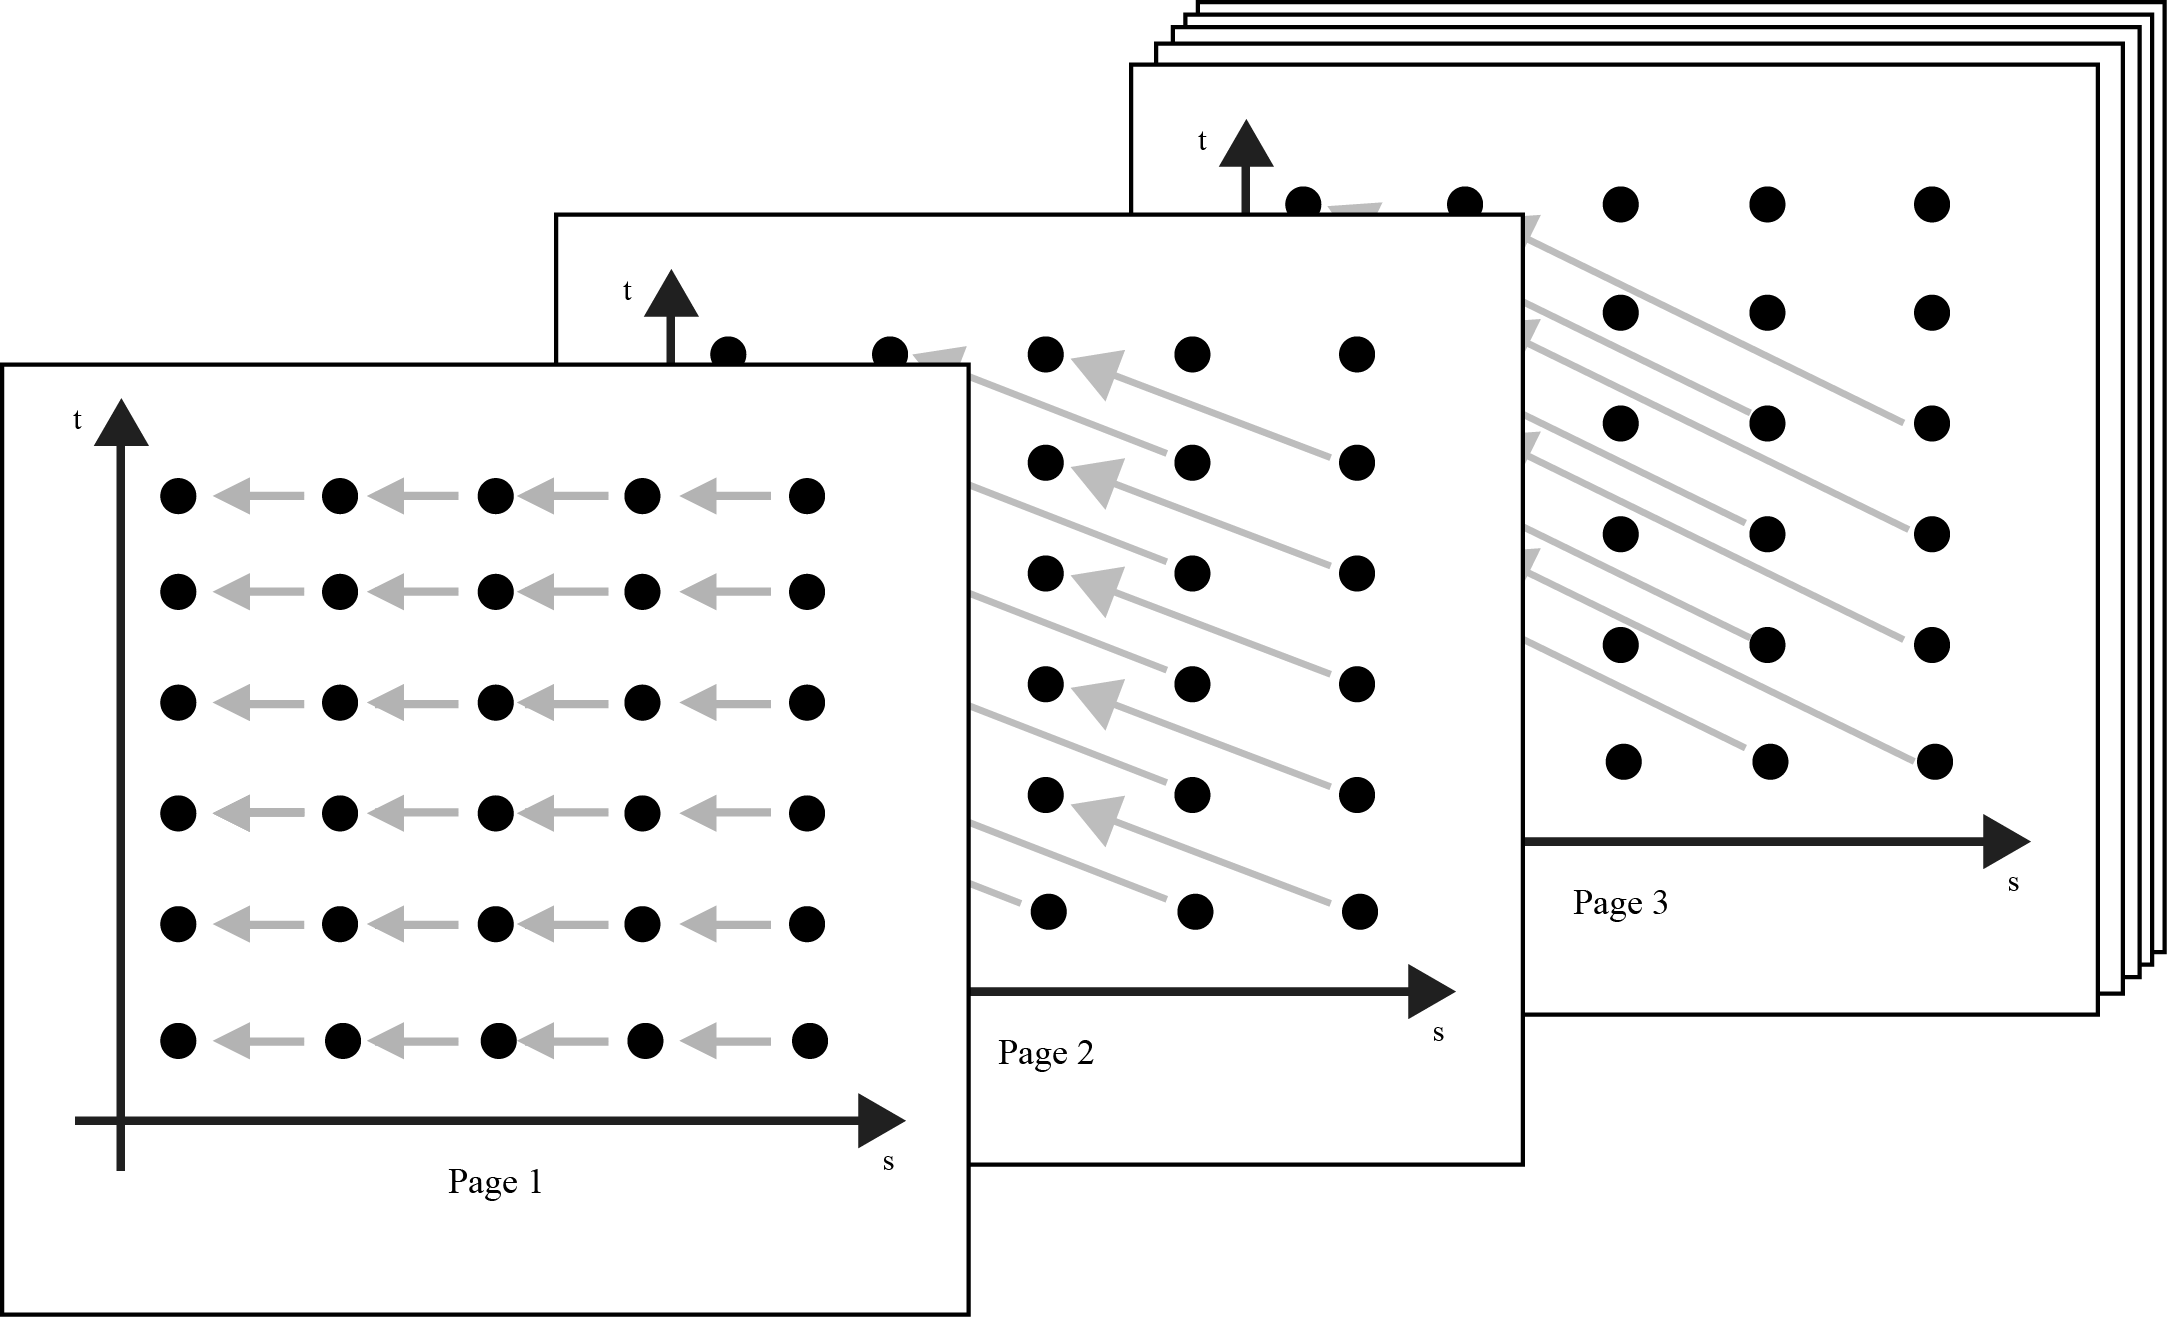
\includegraphics[width=\linewidth,height=0.45\textheight,keepaspectratio]{figures/cover.png}
  \end{center}
       \begin{minipage}{.35\linewidth}
    \begin{flushleft}
      \vspace{2em}
      {\fontsize{6pt}{2pt} \textit{Notes: These are notes live-tex'd
from a graduate course in 4-Manifolds taught by Philip Engel at the
University of Georgia in Spring 2021. As such, any errors or
inaccuracies are almost certainly my own. } } \\
    \end{flushleft}
    \end{minipage}
    \hfill
    \begin{minipage}{.65\linewidth}
    \end{minipage}
  }







\begin{document}

\date{}
\author{D. Zack Garza}
\maketitle
\begin{flushleft}
\textit{D. Zack Garza} \\
\textit{University of Georgia} \\
  \textit{\href{mailto: dzackgarza@gmail.com}{dzackgarza@gmail.com}} \\
{\tiny \textit{Last updated:} 2021-01-28 }
\end{flushleft}


\newpage

% Note: addsec only in KomaScript
\addsec{Table of Contents}
\tableofcontents
\newpage

\def\contradiction
{
\tikz[baseline, x=0.2em, y=0.2em, line width=0.04em]
\draw (0,0) -- ({4*cos(45)},{4*sin(45)})
    (-1,1) -- ({-1 + 4*cos(45)},{1 + 4*sin(45)})
    (-1,3) -- ({-1 + 4*cos(315)},{3 + 4*sin(315)})
    (0,4) -- ({0 + 4*cos(315)},{4 + 4*sin(315)});
}

\hypertarget{tuesday-january-12}{%
\section{Tuesday, January 12}\label{tuesday-january-12}}

\hypertarget{background}{%
\subsection{Background}\label{background}}

From Phil's email:

There are very few references in the notes, and I'll try to update them
to include more as we go. Personally, I found the following online
references particularly useful:

\begin{itemize}
\item
  Dietmar Salamon: Spin Geometry and Seiberg-Witten Invariants
  \autocite{Dietmar99}
\item
  Richard Mandelbaum: Four-dimensional Topology: An Introduction
  \autocite{Mandelbaum1980}

  \begin{itemize}
  \tightlist
  \item
    This book has a nice introduction to surgery aspects of
    four-manifolds, but as a warning: It was published right before
    Freedman's famous theorem. For instance, the existence of an exotic
    R\^{}4 was not known. This actually makes it quite useful, as a
    summary of what was known before, and provides the historical
    context in which Freedman's theorem was proven.
  \end{itemize}
\item
  Danny Calegari: Notes on 4-Manifolds \autocite{Calegari}
\item
  Yuli Rudyak: Piecewise Linear Structures on Topological Manifolds
  \autocite{Rudyak}
\item
  Akhil Mathew: The Dirac Operator \autocite{Matthew}
\item
  Tom Weston: An Introduction to Cobordism Theory \autocite{Weston}

  A wide variety of lecture notes on the Atiyah-Singer index theorem,
  which are available online.
\end{itemize}

\hypertarget{introduction}{%
\subsection{Introduction}\label{introduction}}

\begin{definition}[Topological Manifold]

Recall that a \textbf{topological manifold} (or \(C^0\) manifold) \(X\)
is a Hausdorff topological space \emph{locally homeomorphic} to
\({\mathbb{R}}^n\) with a countable topological base, so we have charts
\(\phi_u: U\to {\mathbb{R}}^n\) which are homeomorphisms from open sets
covering \(X\).

\end{definition}

\begin{example}[The circle]

\(S^1\) is covered by two charts homeomorphic to intervals:

\begin{figure}
\centering
\resizebox{\columnwidth}{!}{%
\begin{tikzpicture}
\node (node_one) at (0,0) { \fontsize{45pt}{1em} \import{/home/zack/SparkleShare/github.com/Notes/Class_Notes/2021/Spring/FourManifolds/sections/figures/}{2021-01-16_21-54.pdf_tex} };
\end{tikzpicture}
}
\end{figure}

\end{example}

\begin{remark}

Maps that are merely continuous are poorly behaved, so we may want to
impose extra structure. This can be done by imposing restrictions on the
transition functions, defined as
\begin{align*}
t_{uv} \coloneqq\varphi_V \to \varphi_U ^{-1} : \varphi_U(U \cap V) \to \varphi_V(U \cap V)
.\end{align*}

\end{remark}

\begin{definition}[Restricted Structures on Manifolds]

\envlist

\begin{itemize}
\item
  We say \(X\) is a \textbf{PL manifold} if and only if \(t_{UV}\) are
  piecewise-linear. Note that an invertible PL map has a PL inverse.
\item
  We say \(X\) is a \textbf{\(C^k\) manifold} if they are \(k\) times
  continuously differentiable, and \textbf{smooth} if infinitely
  differentiable.
\item
  We say \(X\) is \textbf{real-analytic} if they are locally given by
  convergent power series.
\item
  We say \(X\) is \textbf{complex-analytic} if under the identification
  \({\mathbb{R}}^n \cong {\mathbb{C}}^{n/2}\) if they are holomorphic,
  i.e.~the differential of \(t_{UV}\) is complex linear.
\item
  We say \(X\) is a \textbf{projective variety} if it is the vanishing
  locus of homogeneous polynomials on \({\mathbb{CP}}^N\).
\end{itemize}

\end{definition}

\begin{remark}

Is this a strictly increasing hierarchy? It's not clear e.g.~that every
\(C^k\) manifold is PL.

\end{remark}

\begin{question}

Consider \({\mathbb{R}}^n\) as a topological manifold: are any two
smooth structures on \({\mathbb{R}}^n\) diffeomorphic?

\end{question}

\begin{remark}

Fix a copy of \({\mathbb{R}}\) and form a single chart
\({\mathbb{R}}\xrightarrow{\operatorname{id}} {\mathbb{R}}\). There is
only a single transition function, the identity, which is smooth. But
consider
\begin{align*}
X &\to {\mathbb{R}}\\
t &\mapsto t^3
.\end{align*}
This is also a smooth structure on \(X\), since the transition function
is the identity. This yields a different smooth structure, since these
two charts don't like in the same maximal atlas. Otherwise there would
be a transition function of the form \(t_{VU}: t\mapsto t^{1/3}\), which
is not smooth at zero. However, the map
\begin{align*}
X &\to X \\
t &\mapsto t^3
.\end{align*}
defines a diffeomorphism between the two smooth structures.

\end{remark}

\begin{claim}

\({\mathbb{R}}\) admits a unique smooth structure.

\end{claim}

\begin{proof}[sketch]

Let \(\tilde {\mathbb{R}}\) be some exotic \({\mathbb{R}}\), i.e.~a
smooth manifold homeomorphic to \({\mathbb{R}}\). Cover this by
coordinate charts to the standard \({\mathbb{R}}\):

\begin{figure}
\centering
\resizebox{\columnwidth}{!}{%
\begin{tikzpicture}
\node (node_one) at (0,0) { \import{/home/zack/SparkleShare/github.com/Notes/Class_Notes/2021/Spring/FourManifolds/sections/figures}{2021-01-16_22-31.pdf_tex} };
\end{tikzpicture}
}
\end{figure}

\begin{fact}

There exists a cover which is \emph{locally finite} and supports a
\emph{partition of unity}: a collection of smooth functions
\(f_i: U_i \to {\mathbb{R}}\) with \(f_i \geq 0\) and
\({\operatorname{supp}}f \subseteq U_i\) such that \(\sum f_i = 1\)
(\emph{i.e., bump functions}). It is also a purely topological fact that
\(\tilde {\mathbb{R}}\) is orientable.

\end{fact}

So we have bump functions:

\begin{figure}
\centering
\resizebox{\columnwidth}{!}{%
\begin{tikzpicture}
\node (node_one) at (0,0) { \import{/home/zack/SparkleShare/github.com/Notes/Class_Notes/2021/Spring/FourManifolds/sections/figures}{2021-01-16_22-37.pdf_tex} };
\end{tikzpicture}
}
\end{figure}

Take a smooth vector field \(V_i\) on \(U_i\) everywhere aligning with
the orientation. Then \(\sum f_i V_i\) is a smooth nowhere vector field
on \(X\) that is nowhere zero in the direction of the orientation.
Taking the associated flow
\begin{align*}
{\mathbb{R}}&\to \tilde {\mathbb{R}}\\
t &\mapsto \varphi(t)
.\end{align*}
such that \(\varphi'(t) = V(\varphi(t))\). Then \(\varphi\) is a smooth
map that defines a diffeomorphism. This follows from the fact that the
vector field is everywhere positive.

\begin{slogan}

To understand smooth structures on \(X\), we should try to solve
differential equations on \(X\).

\end{slogan}

\end{proof}

\begin{remark}

Note that here we used the existence of a global frame, i.e.~a
trivialization of the tangent bundle, so this doesn't quite work for
e.g.~\(S^2\).

\end{remark}

\begin{question}

What is the difference between all of the above structures? Are there
obstructions to admitting any particular one?

\end{question}

\begin{answer}

\envlist

\begin{enumerate}
\def\labelenumi{\arabic{enumi}.}
\item
  (Munkres) Every \(C^1\) structure gives a unique \(C^k\) and
  \(C^ \infty\) structure.\footnote{Note that this doesn't start at
    \(C^0\), so topological manifolds are genuinely different! There
    exist topological manifolds with no smooth structure.}
\item
  (Grauert) Every \(C^ \infty\) structure gives a unique real-analytic
  structure.
\item
  Every PL manifold admits a smooth structure in \(\dim X \leq 7\), and
  it's unique in \(\dim X\leq 6\), and above these dimensions there
  exists PL manifolds with no smooth structure.
\item
  (Kirby--Siebenmann) Let \(X\) be a topological manifold of
  \(\dim X\geq 5\), then there exists a cohomology class
  \(\operatorname{ks}(X) \in H^4(X; {\mathbb{Z}}/2{\mathbb{Z}})\) which
  is 0 if and only if \(X\) admits a PL structure. Moreover, if
  \(\operatorname{ks}(X) = 0\), then (up to concordance) the set of PL
  structures is given by \(H^3(X; {\mathbb{Z}}/2{\mathbb{Z}})\).
\item
  (Moise) Every topological manifold in \(\dim X\leq 3\) admits a unique
  smooth structure.
\item
  (Smale et al.): In \(\dim X\geq 5\), the number of smooth structures
  on a topological manifold \(X\) is finite. In particular,
  \({\mathbb{R}}^n\) for \(n \neq 4\) has a unique smooth structure. So
  dimension 4 is interesting!
\item
  (Taubes) \({\mathbb{R}}^4\) admits uncountably many non-diffeomorphic
  smooth structures.
\item
  A compact oriented smooth surface \(\Sigma\), the space of
  complex-analytic structures is a complex orbifold \footnote{Locally
    admits a chart to \({\mathbb{C}}^n/ \Gamma\) for \(\Gamma\) a finite
    group.} of dimension \(3g-2\) where \(g\) is the genus of
  \(\Sigma\), up to biholomorphism (i.e.~\emph{moduli}).
\end{enumerate}

\end{answer}

\begin{remark}

Kervaire-Milnor: \(S^7\) admits 28 smooth structures, which form a
group.

\end{remark}

\hypertarget{friday-january-15}{%
\section{Friday, January 15}\label{friday-january-15}}

\begin{remark}

Let
\begin{align*}
V &\coloneqq\left\{{a^2 + b^2 + c^2 + d^3 + e^{6k-1} = 0}\right\} \subseteq {\mathbb{C}}^5 \\
S_\varepsilon&\coloneqq\left\{{ {\left\lvert {a} \right\rvert}^2 + {\left\lvert {b} \right\rvert}^2 + {\left\lvert {c} \right\rvert}^2 + {\left\lvert {d} \right\rvert}^2 + {\left\lvert {e} \right\rvert}^2}\right\}
.\end{align*}
Then \(V_k \cap S_\varepsilon\cong S^7\) is a homeomorphism, and taking
\(k=1,2,\cdots, 28\) yields the 28 smooth structures on \(S^7\). Note
that \(V_k\) is the cone over \(V_k \cap S_\varepsilon\).

\begin{figure}
\centering
\resizebox{\columnwidth}{!}{%
\begin{tikzpicture}
\node (node_one) at (0,0) { 
\fontsize{25pt}{1em} 
\import{/home/zack/SparkleShare/github.com/Notes/Class_Notes/2021/Spring/FourManifolds/sections/figures/}{2021-01-15_13-54.pdf_tex} };
\end{tikzpicture}
}
\end{figure}

\begin{quote}
? Admits a smooth structure, and
\(\mkern 1.5mu\overline{\mkern-1.5muV\mkern-1.5mu}\mkern 1.5mu_k \subseteq {\mathbb{CP}}^5\)
admits no smooth structure.
\end{quote}

\end{remark}

\begin{question}

Is every triangulable manifold PL, i.e.~homeomorphic to a simplicial
complex?

\end{question}

\begin{answer}

No! Given a simplicial complex, there is a notion of the
\textbf{combinatorial link} \(L_V\) of a vertex \(V\):

\begin{figure}
\centering
\resizebox{\columnwidth}{!}{%
\begin{tikzpicture}
\node (node_one) at (0,0) {
\import{/home/zack/SparkleShare/github.com/Notes/Class_Notes/2021/Spring/FourManifolds/sections/figures/}{2021-01-15_13-57.pdf_tex} };
\end{tikzpicture}
}
\end{figure}

It turns out that there exist simplicial manifolds such that the link is
not homeomorphic to a sphere, whereas every PL manifold admits a ``PL
triangulation'' where the links are spheres.

\end{answer}

\begin{remark}

What's special in dimension 4? Recall the \textbf{Kirby-Siebenmann}
invariant \(\operatorname{ks}(x) \in H^4(X; {\mathbb{Z}}_2)\) for \(X\)
a topological manifold where \(\operatorname{ks}(X) = 0 \iff X\) admits
a PL structure, with the caveat that \(\dim X \geq 5\). We can use this
to cook up an invariant of 4-manifolds.

\end{remark}

\begin{definition}[Kirby-Siebenmann Invariant of a 4-manifold]

Let \(X\) be a topological 4-manifold, then
\begin{align*}
\operatorname{ks}(X) \coloneqq\operatorname{ks}(X \times{\mathbb{R}})
.\end{align*}

\end{definition}

\begin{remark}

Recall that in \(\dim X\geq 7\), every PL manifold admits a smooth
structure, and we can note that
\begin{align*}
H^4(X; {\mathbb{Z}}_2) = H^4(X \times{\mathbb{R}}; {\mathbb{Z}}_2) = {\mathbb{Z}}_2,
.\end{align*}
since every oriented 4-manifold admits a fundamental class. Thus
\begin{align*}
\operatorname{ks}(X) = 
\begin{cases}
0 & X \times{\mathbb{R}}\text{ admits a PL and smooth structure} 
\\
1 & X \times{\mathbb{R}}\text{ admits no PL or smooth structures }.
\end{cases}
\end{align*}

\end{remark}

\begin{remark}

\(\operatorname{ks}(X) \neq 0\) implies that \(X\) has no smooth
structure, since \(X \times{\mathbb{R}}\) doesn't. Note that it was not
known if this invariant was nonzero for a while!

\end{remark}

\begin{remark}

Note that \(H^2(X; {\mathbb{Z}})\) admits a symmetric bilinear form
\(Q_X\) defined by
\begin{align*}
{\left\langle { \alpha},~{ \beta} \right\rangle} \mapsto \int_X \alpha\wedge \beta = \alpha \smile\beta([X]) \in {\mathbb{Z}}
.\end{align*}
where \([X]\) is the fundamental class.

\end{remark}

\hypertarget{main-theorems-for-the-course}{%
\section{Main Theorems for the
Course}\label{main-theorems-for-the-course}}

Proving the following theorems is the main goal of this course.

\begin{theorem}[Freedman]

If \(X, Y\) are compact oriented topological 4-manifolds, then
\(X\cong Y\) are homeomorphic if and only if
\(\operatorname{ks}(X) = \operatorname{ks}(Y)\) and \(Q_X \cong Q_Y\)
are isometric, i.e.~there exists an isometry
\begin{align*}
\varphi: H^2(X; {\mathbb{Z}}) \to H^2(Y; {\mathbb{Z}})
.\end{align*}
that preserves the two bilinear forms in the sense that
\({\left\langle {\varphi \alpha},~{ \varphi \beta} \right\rangle} = {\left\langle { \alpha},~{ \beta} \right\rangle}\).

Conversely, every \textbf{unimodular} bilinear form appears as
\(H^2(X; {\mathbb{Z}})\) for some \(X\), i.e.~the pairing induces a map
\begin{align*}
H^2(X; {\mathbb{Z}}) &\to H^2(X; {\mathbb{Z}})^\vee\\
\alpha \mapsto {\left\langle { \alpha },~{ {\,\cdot\,}} \right\rangle}
.\end{align*}
which is an isomorphism. This is essentially a classification of
simply-connected 4-manifolds.

\end{theorem}

\begin{remark}

Note that preservation of a bilinear form is a stand-in for ``being an
element of the orthogonal group'', where we only have a lattice instead
of a full vector space.

\end{remark}

\begin{remark}

There is a map
\(H^2(X; {\mathbb{Z}}) \xrightarrow{PD} H_2(X; {\mathbb{Z}})\) from
Poincaré , where we can think of elements in the latter as closed
surfaces \([\Sigma]\), and
\begin{align*}
{\left\langle { \Sigma_1 },~{ \Sigma_2 } \right\rangle} = \text{signed number of intersections points of } \Sigma_1 \pitchfork\Sigma_2
.\end{align*}
Note that Freedman's theorem is only about homeomorphism, and is not
true smoothly. This gives a way to show that two 4-manifolds are
homeomorphic, but this is hard to prove! So we'll black-box this, and
focus on ways to show that two \emph{smooth} 4-manifolds are \emph{not}
diffeomorphic, since we want homeomorphic but non-diffeomorphic
manifolds.

\end{remark}

\begin{definition}[Signature]

The \textbf{signature} of a topological 4- manifold is the signature of
\(Q_X\), where we note that \(Q_X\) is a symmetric nondegenerate
bilinear form on \(H^2(X; {\mathbb{R}})\) and for some \(a, b\)
\begin{align*}
(H^2(X; {\mathbb{R}}), Q_x) \xrightarrow{\text{isometric}} {\mathbb{R}}^{a, b}
.\end{align*}
where \(a\) is the number of \(+1\)s appearing in the matrix and \(b\)
is the number of \(-1\)s. This is \({\mathbb{R}}^{ab}\) where
\(e_i^2 = 1, i=1\cdots a\) and \(e_i^2 = -1, i=a+1, \cdots b\), and is
thus equipped with a specific bilinear form corresponding to the Gram
matrix of this basis.
\begin{align*}
\begin{bmatrix}
1 & 0 & 0 & 0 & 0
\\
0 & 1 & 0 & 0 & 0
\\
0 & 0 & \ddots & 0 & 0
\\
0 & 0 & 0 & -1 & 0
\\
0 & 0 & 0 & 0 & -1
\end{bmatrix}
= I_{a\times a} \oplus -I_{b \times b}
.\end{align*}
Then the signature is \(a-b\), the dimension of the positive-definite
space minus the dimension of the negative-definite space.

\end{definition}

\begin{theorem}[Rokhlin's Theorem]

Suppose
\({\left\langle { \alpha},~{\alpha} \right\rangle} \in 2{\mathbb{Z}}\)
and \(\alpha\in H^2(X; {\mathbb{Z}})\) and \(X\) a simply connected
\textbf{smooth} 4-manifold. Then 16 divides \(\operatorname{sig}(X)\).

\end{theorem}

\begin{remark}

Note that Freedman's theorem implies that there exists topological
4-manifolds with no smooth structure.

\end{remark}

\begin{theorem}[Donaldson]

Let \(X\) be a smooth simply-connected 4-manifold. If \(a=0\) or
\(b=0\), then \(Q_X\) is diagonalizable and there exists an orthonormal
basis of \(H^2(X; {\mathbb{Z}})\).

\end{theorem}

\begin{remark}

This comes from Gram-Schmidt, and restricts what types of intersection
forms can occur.

\end{remark}

\hypertarget{warm-up-mathbbr2-has-a-unique-smooth-structure}{%
\subsection{\texorpdfstring{Warm Up: \({\mathbb{R}}^2\) Has a Unique
Smooth
Structure}{Warm Up: \{\textbackslash mathbb\{R\}\}\^{}2 Has a Unique Smooth Structure}}\label{warm-up-mathbbr2-has-a-unique-smooth-structure}}

\begin{remark}

Last time we showed \({\mathbb{R}}^1\) had a unique smooth structure, so
now we'll do this for \({\mathbb{R}}^2\). The strategy of solving a
differential equation, we'll now sketch the proof.

\end{remark}

\begin{definition}[Riemannian Metrics]

A \textbf{Riemannian metric} \(g\in \operatorname{Sym}^2 T^*X\) for
\(X\) a smooth manifold is a metric on every \(T_p X\) given by
\begin{align*}
g_p: T_pX \times T_p X &\to {\mathbb{R}}\\
g(v, v) \geq 0, g(v,v) = 0 \iff v=0
.\end{align*}

\end{definition}

\begin{definition}[Almost complex structure]

An \textbf{almost complex structure} is a
\(J\in \mathop{\mathrm{End}}(TX)\) such that
\(J^2 = -\operatorname{id}\).

\end{definition}

\begin{remark}

Let \(e\in T_p X\) and \(e\neq 0\), then if \(X\) is a surface then
\(\left\{{e, Je}\right\}\) is a basis of \(T_p X\).

\begin{figure}
\centering
\resizebox{\columnwidth}{!}{%
\begin{tikzpicture}
\node (node_one) at (0,0) { 
\fontsize{25pt}{1em} 
\import{/home/zack/SparkleShare/github.com/Notes/Class_Notes/2021/Spring/FourManifolds/sections/figures/}{2021-01-15_14-33.pdf_tex} };
\end{tikzpicture}
}
\end{figure}

This is a basis because if \(Je\) and \(e\) are parallel, then ??? In
particular, \(J_p\) is determined by a point in
\({\mathbb{R}}^2\setminus\left\{{\text{the }x{\hbox{-}}\text{axis}}\right\}\)

\end{remark}

\hypertarget{sketch-of-proof}{%
\subsubsection{Sketch of Proof}\label{sketch-of-proof}}

Let \(\tilde {\mathbb{R}}^2\) be an exotic \({\mathbb{R}}^2\).

\hypertarget{step-1}{%
\paragraph{Step 1}\label{step-1}}

Choose a metric on \(\tilde {\mathbb{R}}^2\) \(g \coloneqq\sum f_I g_i\)
with \(g_i\) metrics on coordinate charts \(U_i\) and \(f_i\) a
partition of unity.

\hypertarget{step-2}{%
\paragraph{Step 2}\label{step-2}}

Find an almost complex structure on \(\tilde {\mathbb{R}}^2\). Choosing
an orientation of \(\tilde {\mathbb{R}}^2\), \(g\) defines a unique
almost complex structure
\(J_p e \coloneqq f\in T_p \tilde {\mathbb{R}}^2\) such that

\begin{itemize}
\tightlist
\item
  \(g(e, e) = g(f, f)\)
\item
  \(g(e, f) = 0\).
\item
  \(\left\{{e, f}\right\}\) is an oriented basis of
  \(T_p \tilde {\mathbb{R}}^2\)
\end{itemize}

This is because after choosing \(e\), there are two orthogonal vectors,
but only one choice yields an \emph{oriented} basis.

\begin{figure}
\centering
\resizebox{\columnwidth}{!}{%
\begin{tikzpicture}
\node (node_one) at (0,0) {
\fontsize{25pt}{1em} 
  \import{/home/zack/SparkleShare/github.com/Notes/Class_Notes/2021/Spring/FourManifolds/sections/figures/}{2021-01-15_14-39.pdf_tex}
  };
\end{tikzpicture}
}
\end{figure}

\hypertarget{step-3}{%
\paragraph{Step 3}\label{step-3}}

We then apply a theorem:

\begin{theorem}[?]

Any almost complex structure on a surface comes from a complex
structure, in the sense that there exist charts
\(\varphi_i: U_i \to {\mathbb{C}}\) such that \(J\) is multiplication by
\(i\).

\end{theorem}

So \(d \varphi(J \cdot e) = i \cdot d \varphi_i (e)\), and
\((\tilde {\mathbb{R}}^2, J)\) is a complex manifold. Since it's simply
connected, the Riemann Mapping Theorem shows that it's biholomorphic to
\({\mathbb{D}}\) or \({\mathbb{C}}\), both of which are diffeomorphic to
\({\mathbb{R}}^2\).

\begin{quote}
See the Newlander-Nirenberg theorem, a result in complex geometry.
\end{quote}

\hypertarget{lecture-3-wednesday-january-20}{%
\section{Lecture 3 (Wednesday, January
20)}\label{lecture-3-wednesday-january-20}}

Today: some background material on sheaves, bundles, connections.

\hypertarget{sheaves}{%
\subsection{Sheaves}\label{sheaves}}

\begin{definition}[Presheaves and Sheaves]

Recall that if \(X\) is a topological space, a \textbf{presheaf} of
abelian groups \(\mathcal{F}\) is an assignment \(U\to \mathcal{F}(U)\)
of an abelian group to every open set \(U \subseteq X\) together with a
restriction map \(\rho_{UV}: \mathcal{F}(U) \to \mathcal{F}(V)\) for any
inclusion \(V \subseteq U\) of open sets. This data has to satisfying
certain conditions:

\begin{enumerate}
\def\labelenumi{\alph{enumi}.}
\item
  \(\mathcal{F}(\emptyset) = 0\), the trivial abelian group.
\item
  \(\rho_{UU}: \mathcal{F}(U) \to \mathcal{F}(U) = \operatorname{id}_{\mathcal{F}(U) }\)
\item
  Compatibility if restriction is taken in steps:
  \(U \subseteq V \subseteq W \implies \rho_{VW} \circ \rho_{UV} = \rho_{UW}\).
\end{enumerate}

We say \(\mathcal{F}\) is a \textbf{sheaf} if additionally:

\begin{enumerate}
\def\labelenumi{\alph{enumi}.}
\setcounter{enumi}{3}
\tightlist
\item
  Given \(s_i \in \mathcal{F}(U_i)\) such that
  \(\rho_{U_i \cap U_j} (s_i) = \rho_{U_i \cap U_j} (s_j)\) implies that
  there exists a unique \(s\in \mathcal{F}(\bigcup_i U_i)\) such that
  \(\rho_{U_i}(s) = s_i\).
\end{enumerate}

\begin{figure}
\centering
\resizebox{\columnwidth}{!}{%
\begin{tikzpicture}
\node (node_one) at (0,0) { 
\fontsize{45pt}{1em} 
\import{/home/zack/SparkleShare/github.com/Notes/Class_Notes/2021/Spring/FourManifolds/sections/figures}{2021-01-20_13-59.pdf_tex} };
\end{tikzpicture}
}
\end{figure}

\end{definition}

\begin{example}[?]

Let \(X\) be a topological manifold, then
\(\mathcal{F}\coloneqq C^0({\,\cdot\,}, {\mathbb{R}})\) the set of
continuous functionals form a sheaf. We have a diagram

\begin{center}
\begin{tikzcd}
    U && {C^0(U; {\mathbb{R}})} \\
    \\
    V && {C^0(V; {\mathbb{R}})}
    \arrow[hook, from=3-1, to=1-1]
    \arrow["{\text{restrict cts. functions}}", dashed, hook, from=1-3, to=3-3]
    \arrow["{\mathcal{F}}", from=1-1, to=1-3]
    \arrow["{\mathcal{F}}"', from=3-1, to=3-3]
\end{tikzcd}
\end{center}

\begin{quote}
\href{https://q.uiver.app/?q=WzAsNCxbMCwwLCJVIl0sWzAsMiwiViJdLFsyLDAsIkNeMChVOyBcXFJSKSJdLFsyLDIsIkNeMChWOyBcXFJSKSJdLFsxLDAsIiIsMCx7InN0eWxlIjp7InRhaWwiOnsibmFtZSI6Imhvb2siLCJzaWRlIjoidG9wIn19fV0sWzIsMywiXFx0ZXh0e3Jlc3RyaWN0IGN0cy4gZnVuY3Rpb25zfSIsMCx7InN0eWxlIjp7InRhaWwiOnsibmFtZSI6Imhvb2siLCJzaWRlIjoidG9wIn0sImJvZHkiOnsibmFtZSI6ImRhc2hlZCJ9fX1dLFswLDIsIlxcbWF0aGNhbHtGfSJdLFsxLDMsIlxcbWF0aGNhbHtGfSIsMl1d}{Link
to diagram}
\end{quote}

Property (d) holds because given sections
\(s_i \in C^0(U_i; {\mathbb{R}})\) agreeing on overlaps, so
\({ \left.{{s_i}} \right|_{{U_i \cap U_j}} } = { \left.{{s_j}} \right|_{{U_i \cap U_j}} }\),
there exists a unique \(s\in C^0(\bigcup_i U_i; {\mathbb{R}})\) such
that \({ \left.{{s}} \right|_{{U_i}} } = s_i\) for all \(i\) --
continuous functions glue.

\end{example}

\begin{remark}

Recall that we discussed various structures on manifolds: PL,
continuous, smooth, complex-analytic, etc. We can characterize these by
their sheaves of functions, which we'll denote \({\mathcal{O}}\). For
example, \({\mathcal{O}}\coloneqq C^0({\,\cdot\,}; {\mathbb{R}})\) for
topological manifolds, and
\({\mathcal{O}}\coloneqq C^ \infty ({\,\cdot\,}; {\mathbb{R}})\) is the
sheaf for smooth manifolds. Note that this also works for PL functions,
since pullbacks of PL functions are again PL. For complex manifolds, we
set \({\mathcal{O}}\) to be the sheaf of holomorphic functions.

\end{remark}

\begin{example}[Locally Constant Sheaves]

Let \(A\in {\operatorname{Ab}}\) be an abelian group, then
\(\underline{A}\) is the sheaf defined by setting \(\underline{A}(U)\)
to be the locally constant functions \(U\to A\). E.g. let
\(X \in {\operatorname{Mfd}}_{{\operatorname{Top}}}\) be a topological
manifold, then \(\underline{{\mathbb{R}}}(U) = {\mathbb{R}}\) if \(U\)
is connected since locally constant \(\implies\) globally constant in
this case.

\end{example}

\begin{warnings}

Note that the presheaf of constant functions doesn't satisfy (d)! Take
\({\mathbb{R}}\) and a function with two different values on disjoint
intervals:

\begin{figure}
\centering
\resizebox{\columnwidth}{!}{%
\begin{tikzpicture}
\node (node_one) at (0,0) { 
\fontsize{41pt}{1em} 
\import{/home/zack/SparkleShare/github.com/Notes/Class_Notes/2021/Spring/FourManifolds/sections/figures}{2021-01-20_14-11.pdf_tex} };
\end{tikzpicture}
}
\end{figure}

Note that
\({ \left.{{s_1}} \right|_{{U_1 \cap U_2}} } = { \left.{{s_2}} \right|_{{U_1 \cap U_2}} }\)
since the intersection is empty, but there is no constant function that
restricts to the two different values.

\end{warnings}

\hypertarget{bundles}{%
\subsection{Bundles}\label{bundles}}

\begin{remark}

Let \(\pi: \mathcal{E}\to X\) be a \textbf{vector bundle}, so we have
local trivializations \(\pi ^{-1} (U) \xrightarrow{h_u} Y^d \times U\)
where we take either \(Y={\mathbb{R}}, {\mathbb{C}}\), such that
\(h_v \circ h_u ^{-1}\) preserves the fibers of \(\pi\) and acts
linearly on each fiber of \(Y\times(U \cap V)\). Define
\begin{align*}
t_{UV}: U \cap V \to \operatorname{GL}_d(Y)
\end{align*}
where we require that \(t_{UV}\) is continuous, smooth,
complex-analytic, etc depending on the context.

\begin{figure}
\centering
\resizebox{\columnwidth}{!}{%
\begin{tikzpicture}
\node (node_one) at (0,0) { 
\fontsize{47pt}{1em} 
\import{/home/zack/SparkleShare/github.com/Notes/Class_Notes/2021/Spring/FourManifolds/sections/figures}{2021-01-20_14-17.pdf_tex} };
\end{tikzpicture}
}
\end{figure}

\end{remark}

\begin{example}[Bundles over $S^1$]

There are two \({\mathbb{R}}^1\) bundles over \(S^1\):

\begin{figure}
\centering
\resizebox{\columnwidth}{!}{%
\begin{tikzpicture}
\node (node_one) at (0,0) { 
\fontsize{32pt}{1em} 
\import{/home/zack/SparkleShare/github.com/Notes/Class_Notes/2021/Spring/FourManifolds/sections/figures}{2021-01-20_14-20.pdf_tex} };
\end{tikzpicture}
}
\end{figure}

Note that the Mobius bundle is not trivial, but can be locally
trivialized.

\end{example}

\begin{remark}

We abuse notation: \(\mathcal{E}\) is also a sheaf, and we write
\(\mathcal{E}(U)\) to be the set of sections \(s: U\to \mathcal{E}\)
where \(s\) is continuous, smooth, holomorphic, etc where
\(\pi \circ s = \operatorname{id}_U\). I.e. a bundle is a sheaf in the
sense that its sections \emph{form} a sheaf.

\end{remark}

\begin{example}[?]

The trivial line bundle gives the sheaf \({\mathcal{O}}\) : maps
\(U \xrightarrow{s} U\times Y\) for \(Y={\mathbb{R}}, {\mathbb{C}}\)
such that \(\pi \circ s = \operatorname{id}\) are the same as maps
\(U\to Y\).

\end{example}

\begin{definition}[$\OO\dash$modules]

An \textbf{\({\mathcal{O}}{\hbox{-}}\)module} is a sheaf \(\mathcal{F}\)
such that \(\mathcal{F}(U)\) has an action of \(\mathcal{O}(U)\)
compatible with restriction.

\end{definition}

\begin{example}[?]

If \(\mathcal{E}\) is a vector bundle, then \(\mathcal{E}(U)\) has a
natural action of \({\mathcal{O}}(U)\) given by
\(f\curvearrowright s \coloneqq fs\), i.e.~just multiplying functions.

\end{example}

\begin{example}[Non-example]

The locally constant sheaf \(\underline{{\mathbb{R}}}\) is not an
\({\mathcal{O}}{\hbox{-}}\)module: there isn't natural action since the
sections of \({\mathcal{O}}\) are generally non-constant functions, and
multiplying a constant function by a non-constant function doesn't
generally give back a constant function.

\end{example}

We'd like a notion of maps between sheaves:

\begin{definition}[Morphisms of Sheaves]

A \textbf{morphism} of sheaves \(\mathcal{F} \to \mathcal{G}\) is a
group morphism \(\varphi(U): \mathcal{F}(U) \to \mathcal{G}(U)\) for all
opens \(U \subseteq X\) such that the diagram involving restrictions
commutes:

\begin{center}
\begin{tikzcd}
\mathcal{F}(U) 
\ar[r, "\phi(U)"] 
\ar[d, "\rho_{UV}"]
&
\mathcal{G}(U) 
\ar[d, "\rho_{UV}"]
\\
\mathcal{F}(V) 
\ar[r, "\phi(V)"] 
&
\mathcal{F}(V) 
\end{tikzcd}
\end{center}

\end{definition}

\begin{example}[An $\OO\dash$module that is not a vector bundle.]

Let \(X = {\mathbb{R}}\) and define the \textbf{skyscraper sheaf} at
\(p \in {\mathbb{R}}\) as
\begin{align*}
{\mathbb{R}}_p(U) \coloneqq
\begin{cases}
{\mathbb{R}}& p\in U 
\\
0 & p\not\in U.
\end{cases}
.\end{align*}

The \({\mathcal{O}}(U){\hbox{-}}\)module structure is given by
\begin{align*}
{\mathcal{O}}(U) \times{\mathcal{O}}(U) &\to {\mathbb{R}}_p(U) \\
(f, s) &\mapsto f(p) s
.\end{align*}
This is not a vector bundle since \({\mathbb{R}}_p(U)\) is not an
infinite dimensional vector space, whereas the space of sections of a
vector bundle is generally infinite dimensional (?). Alternatively,
there are arbitrarily small punctured open neighborhoods of \(p\) for
which the sheaf makes trivial assignments.

\end{example}

\begin{example}[of morphisms]

Let \(X = {\mathbb{R}}\in {\operatorname{Mfd}}_{\operatorname{Sm}}\)
viewed as a smooth manifold, then multiplication by \(x\) induces a
morphism of structure sheaves:
\begin{align*}
(x \cdot): {\mathcal{O}}&\to {\mathcal{O}}\\
s & \mapsto x\cdot s
\end{align*}
for any \(x\in {\mathcal{O}}(U)\), noting that
\(x\cdot s\in {\mathcal{O}}(U)\) again.

\begin{exercise}[?]

Check that \(\ker \varphi\) is naturally a sheaf and
\(\ker(\varphi)(U) = \ker (\varphi(U)): \mathcal{F}(U) \to \mathcal{G}(U)\)

\end{exercise}

Here the kernel is trivial, i.e.~on any open \(U\) we have
\((x\cdot):{\mathcal{O}}(U) \hookrightarrow{\mathcal{O}}(U)\) is
injective. Taking the cokernel \(\operatorname{coker}(x\cdot)\) as a
presheaf, this assigns to \(U\) the quotient presheaf
\({\mathcal{O}}(U) / x{\mathcal{O}}(U)\), which turns out to be equal to
\({\mathbb{R}}_0\). So \({\mathcal{O}}\to {\mathbb{R}}_0\) by
restricting to the value at \(0\), and there is an exact sequence
\begin{align*}
0 \to {\mathcal{O}}\xrightarrow{(x\cdot)} {\mathcal{O}}\to {\mathbb{R}}_0 \to 0
.\end{align*}

This is one reason sheaves are better than vector bundles: the category
is closed under taking quotients, whereas quotients of vector bundles
may not be vector bundles.

\end{example}

\hypertarget{lecture-4-friday-january-22}{%
\section{Lecture 4 (Friday, January
22)}\label{lecture-4-friday-january-22}}

\hypertarget{the-exponential-exact-sequence}{%
\subsection{The Exponential Exact
Sequence}\label{the-exponential-exact-sequence}}

Let \(X = {\mathbb{C}}\) and consider \({\mathcal{O}}\) the sheaf of
holomorphic functions and \({\mathcal{O}}^{\times}\) the sheaf of
\emph{nonvanishing} holomorphic functions. The former is a vector bundle
and the latter is a sheaf of abelian groups. There is a map
\(\exp: {\mathcal{O}}\to {\mathcal{O}}^{\times}\), the
\textbf{exponential map}, which is the data
\(\exp(U): {\mathcal{O}}(U) \to {\mathcal{O}}^{\times}(U)\) on every
open \(U\) given by \(f\mapsto e^f\). There is a kernel sheaf
\(2\pi i \underline{{\mathbb{Z}}}\), and we get an exact sequence
\begin{align*}
0 \to 2\pi i \underline{{\mathbb{Z}}} \to {\mathcal{O}}\xrightarrow{\exp} {\mathcal{O}}^{\times}\to \operatorname{coker}(\exp) \to 0
.\end{align*}

\begin{question}

What is the cokernel sheaf here?

\end{question}

Let \(U\) be a contractible open set, then we can identify
\({\mathcal{O}}^{\times}(U) / \exp({\mathcal{O}}^{\times}(U)) = 1\).

\begin{figure}
\centering
\resizebox{\columnwidth}{!}{%
\begin{tikzpicture}
\node (node_one) at (0,0) { 
\fontsize{44pt}{1em} 
\import{/home/zack/SparkleShare/github.com/Notes/Class_Notes/2021/Spring/FourManifolds/sections/figures}{2021-01-22_13-58.pdf_tex} 
};
\end{tikzpicture}
}
\end{figure}

Any \(f\in {\mathcal{O}}^{\times}(U)\) has a logarithm, say by taking a
branch cut, since \(\pi_1(U) =0 \implies \log f\) has an analytic
continuation. Consider the annulus \(U\) and the function
\(z\in {\mathcal{O}}^{\times}(U)\), then
\(z\not\in \exp({\mathcal{O}}(U))\) -- if \(z=e^f\) then \(f=\log(z)\),
but \(\log(z)\) has monodromy on \(U\):

\begin{figure}
\centering
\resizebox{\columnwidth}{!}{%
\begin{tikzpicture}
\node (node_one) at (0,0) { 
\fontsize{44pt}{1em} 
\import{/home/zack/SparkleShare/github.com/Notes/Class_Notes/2021/Spring/FourManifolds/sections/figures}{2021-01-22_14-02.pdf_tex} 
};
\end{tikzpicture}
}
\end{figure}

Thus on any sufficiently small open set,
\(\operatorname{coker}(\exp) = 1\). This is only a presheaf: there
exists an open cover of the annulus for which
\({ \left.{{z}} \right|_{{U_i}} }\), and so the naive cokernel doesn't
define a sheaf. This is because we have a locally trivial section which
glues to \(z\), which is nontrivial.

\begin{exercise}[?]

Redefine the cokernel so that it is a sheaf. Hint: look at
sheafification, which has the defining property
\({\operatorname{Hom}}_{{\operatorname{Presh}}}(\mathcal{G}, \mathcal{F}^{\operatorname{Presh}}) ={\operatorname{Hom}}_{{\operatorname{Sh}}}( \mathcal{G}, \mathcal{F}^{{\operatorname{Sh}}})\)
for any sheaf \(\mathcal{G}\).

\end{exercise}

\begin{definition}[Global Sections Sheaf]

The \textbf{global sections} sheaf of \(\mathcal{F}\) on \(X\) is given
by \(H^0( X; \mathcal{F}) = \mathcal{F}(X)\).

\end{definition}

\begin{example}[?]

\envlist

\begin{itemize}
\tightlist
\item
  \(C^ \infty (X) = H^0(X, C^ \infty )\) are the smooth functions on
  \(X\)
\item
  \(VF(X) = H^0(X; T)\) are the smooth vector fields on \(X\) for \(T\)
  the tangent bundle
\item
  If \(X\) is a complex manifold then
  \({\mathcal{O}}(X) = H^0(X; {\mathcal{O}})\) are the globally
  holomorphic functions on \(X\).
\item
  \(H^0(X; {\mathbb{Z}}) = \underline{{\mathbb{Z}}}(X)\) are ??
\end{itemize}

\end{example}

\begin{remark}

Given vector bundles \(V, W\), we have constructions
\(V \oplus W, V \otimes W, V^\vee, {\operatorname{Hom}}(V, W) = V^\vee\otimes W, \operatorname{Sym}^n V, \Lambda^p V\),
and so on. Some of these work directly for sheaves:

\begin{itemize}
\tightlist
\item
  \(\mathcal{F} \oplus \mathcal{G}(U) \coloneqq\mathcal{F}(U) \oplus \mathcal{G}(U)\)
\item
  For tensors, duals, and homs
  \(\mathscr{H}\kern-2pt\operatorname{om}(V, W)\) we only get
  presheaves, so we need to sheafify.
\end{itemize}

\end{remark}

\begin{warnings}

\({\operatorname{Hom}}(V, W)\) will denote the \emph{global}
homomorphisms \(\mathscr{H}\kern-2pt\operatorname{om}(V, W)(X)\), which
is a sheaf.

\end{warnings}

\begin{example}[?]

Let \(X^n \in {\operatorname{Mfd}}_{{\operatorname{sm}}}\) and let
\(\Omega^p\) be the sheaf of smooth \(p{\hbox{-}}\)forms, i.e
\(\Lambda^p T^\vee\), i.e.~\(\Omega^p(U)\) are the smooth \(p\) forms on
\(U\), which are locally of the form
\(\sum f_{i_1, \cdots, i_p} (x_1, \cdots, x_n) dx_{i_1} \wedge dx_{i_2} \wedge \cdots dx_{i_p}\)
where the \(f_{i_1, \cdots, i_p}\) are smooth functions.

\begin{example}[Sub-example]

Take \(X= S^1\), writing this as \({\mathbb{R}}/{\mathbb{Z}}\), we have
\(\Omega^1(X) \ni dx\). There are two coordinate charts which differ by
a translation on their overlaps, and \(dx(x + c) =dx\) for \(c\) a
constant:

\begin{figure}
\centering
\resizebox{\columnwidth}{!}{%
\begin{tikzpicture}
\node (node_one) at (0,0) { 
\fontsize{44pt}{1em} 
\import{/home/zack/SparkleShare/github.com/Notes/Class_Notes/2021/Spring/FourManifolds/sections/figures}{2021-01-22_14-22.pdf_tex} 
};
\end{tikzpicture}
}
\end{figure}

\end{example}

\begin{exercise}[?]

Check that on a torus, \(dx_i\) is a well-defined 1-form.

\end{exercise}

\end{example}

\begin{remark}

Note that there is a map \(d: \Omega^p \to \Omega^{p+1}\) where
\(\omega\mapsto d \omega\).

\end{remark}

\begin{warnings}

\(d\) is \textbf{not} a map of \({\mathcal{O}}{\hbox{-}}\)modules:
\(d(f\cdot \omega) = f\cdot \omega + {\color{red} df \wedge \omega}\),
where the latter is a correction term. In particular, it is not a map of
vector bundles, but is a map of sheaves of abelian groups since
\(d ( \omega_1 + \omega_2) = d( \omega_1 ) + d ( \omega_2)\), making
\(d\) a sheaf morphism.

\end{warnings}

Let \(X \in {\operatorname{Mfd}}_{\mathbb{C}}\), we'll use the fact that
\(TX\) is complex-linear and thus a \({\mathbb{C}}{\hbox{-}}\)vector
bundle.

\begin{figure}
\centering
\resizebox{\columnwidth}{!}{%
\begin{tikzpicture}
\node (node_one) at (0,0) { 
\fontsize{44pt}{1em} 
\import{/home/zack/SparkleShare/github.com/Notes/Class_Notes/2021/Spring/FourManifolds/sections/figures}{2021-01-22_14-27.pdf_tex} 
};
\end{tikzpicture}
}
\end{figure}

\begin{remark}[Subtlety 1]

Note that \(\Omega^p\) for complex manifolds is \(\Lambda^p T^\vee\),
and so if we want to view \(X \in {\operatorname{Mfd}}_{\mathbb{R}}\)
we'll write \(X_{{\mathbb{R}}}\). \(TX_{\mathbb{R}}\) is then a real
vector bundle of rank \(2n\).

\end{remark}

\begin{remark}[Subtlety 2]

\(\Omega^p\) will denote \emph{holomorphic} \(p{\hbox{-}}\)forms,
i.e.~local expressions \(\sum f_I(z_1, \cdots, z_n) \Lambda dz_I\). For
example, \(e^zdz\in \Omega^1({\mathbb{C}})\) but
\(z\mkern 1.5mu\overline{\mkern-1.5muz\mkern-1.5mu}\mkern 1.5mu dz\) is
not, where \(dz = dx + idy\). We'll use a different notation when we
allow the \(f_I\) to just be smooth: \(A^{p, 0}\), the sheaf of
\((p, 0){\hbox{-}}\)forms. Then
\(z\mkern 1.5mu\overline{\mkern-1.5muz\mkern-1.5mu}\mkern 1.5mu dz\in A^{1, 0}\).

\end{remark}

\begin{remark}

Note that
\(T^\vee X_{\mathbb{R}}\otimes _{\mathbb{C}}= A^{1, 0} \oplus A^{0, 1}\)
since there is a unique decomposition
\(\omega = fdz + gd\mkern 1.5mu\overline{\mkern-1.5muz\mkern-1.5mu}\mkern 1.5mu\)
where \(f,g\) are smooth. Then
\(\Omega^d X_{\mathbb{R}}\otimes_{\mathbb{R}}{\mathbb{C}}= \bigoplus _{p+q=d} A^{p, q}\).
Note that \(\Omega_{\setminus}^p \neq A^{p, q}\) and these are really
quite different: the former are more like holomorphic bundles, and the
latter smooth. Moreover \(\dim \Omega^p(X) < \infty\), whereas
\(\Omega_{\setminus}^1\) is infinite-dimensional.

\end{remark}

\hypertarget{principal-ghbox-bundles-and-connections-monday-january-25}{%
\section{\texorpdfstring{Principal \(G{\hbox{-}}\)Bundles and
Connections (Monday, January
25)}{Principal G\{\textbackslash hbox\{-\}\}Bundles and Connections (Monday, January 25)}}\label{principal-ghbox-bundles-and-connections-monday-january-25}}

\begin{definition}[Principal Bundles]

Let \(G\) be a (possibly disconnected) Lie group. Then a
\textbf{principal \(G{\hbox{-}}\)bundle} \(\pi:P\to X\) is a space
admitting local trivializations \(h_u: \pi ^{-1} (U) \to G \times U\)
such that the transition functions are given by left multiplication by a
continuous function \(t_{UV}: U \cap V \to G\).

\begin{figure}
\centering
\resizebox{\columnwidth}{!}{%
\begin{tikzpicture}
\fontsize{40pt}{1em} 
\node (node_one) at (0,0) { \import{/home/zack/SparkleShare/github.com/Notes/Class_Notes/2021/Spring/FourManifolds/sections/figures}{2021-01-25_13-55.pdf_tex} };
\end{tikzpicture}
}
\end{figure}

\end{definition}

\begin{remark}

Setup: we'll consider \(TX\) for
\(X\in {\operatorname{Mfd}}_\setminus\), and let \(g\) be a metric on
the tangent bundle given by
\begin{align*}
g_p: T_pX^{\otimes 2} \to {\mathbb{R}}
,\end{align*}
a symmetric bilinear form with \(g_p(u, v) \geq 0\) with equality if and
only if \(v=0\).

\end{remark}

\begin{definition}[The Frame Bundle]

Define
\({\operatorname{Frame}}_p(X) \coloneqq\left\{{\text{bases of } T_p X}\right\}\),
and
\({\operatorname{Frame}}X \coloneqq\bigcup_{p\in X} {\operatorname{Frame}}_p X\).

\end{definition}

\begin{remark}

More generally, \({\operatorname{Frame}}\mathcal{E}\) can be defined for
any vector bundle \(\mathcal{E}\), so
\({\operatorname{Frame}}X \coloneqq{\operatorname{Frame}}TX\). Note that
\({\operatorname{Frame}}X\) is a principal
\(\operatorname{GL}_n({\mathbb{R}}){\hbox{-}}\)bundle where
\(n\coloneqq\operatorname{rank}(\mathcal{E})\). This follows from the
fact that the transition functions are fiberwise in
\(\operatorname{GL}_n({\mathbb{R}})\), so the transition functions are
given by left-multiplication by matrices.

\end{remark}

\begin{remark}[Important]

A principal \(G{\hbox{-}}\)bundle admits a \(G{\hbox{-}}\)action where
\(G\) acts by \emph{right} multiplication:
\begin{align*}
P \times G \to P \\
( (g, x), h) \mapsto (gh, x)
.\end{align*}
This is necessary for compatibility on overlaps. \textbf{Key point}: the
actions of left and right multiplication commute.

\end{remark}

\begin{definition}[Orthogonal Frame Bundle]

The \textbf{orthogonal frame bundle} of a vector bundle \(\mathcal{E}\)
equipped with a metric \(g\) is defined as
\({\operatorname{OFrame}}_p \mathcal{E}\coloneqq\left\{{\text{orthonormal bases of } \mathcal{E}_p}\right\}\),
also written \(O_r({\mathbb{R}})\) where
\(r \coloneqq\operatorname{rank}( \mathcal{E})\).

\end{definition}

\begin{remark}

The fibers \(P_x \to \left\{{x}\right\}\) of a principal
\(G{\hbox{-}}\)bundle are naturally \textbf{torsors} over \(G\), i.e.~a
set with a free transitive \(G{\hbox{-}}\)action.

\end{remark}

\begin{definition}[?]

Let \(\mathcal{E}\to X\) be a complex vector bundle. Then a
\textbf{hermitian metric} is a hermitian form on every fiber, i.e.~
\begin{align*}
h_p: \mathcal{E}_p \times\overline{\mathcal{E}_p } \to {\mathbb{C}}
.\end{align*}
where
\(h_p(v, \mkern 1.5mu\overline{\mkern-1.5muv\mkern-1.5mu}\mkern 1.5mu ) \geq 0\)
with equality if and only if \(v=0\). Here we define
\(\overline{\mathcal{E}_p}\) as the fiber of the complex vector bundle
\(\overline{\mathcal{E}}\) whose transition functions are given by the
complex conjugates of those from \(\mathcal{E}\).

\end{definition}

\begin{remark}

Note that \(\mathcal{E}, \overline{\mathcal{E}}\) are genuinely
different as complex bundles. There is a \emph{conjugate-linear} map
given by conjugation,
i.e.~\(L(cv) = \mkern 1.5mu\overline{\mkern-1.5muc\mkern-1.5mu}\mkern 1.5mu L(v)\),
where the canonical example is
\begin{align*}
{\mathbb{C}}^n &\to {\mathbb{C}}^n \\
(z_1, \cdots, z_n) &\mapsto (\mkern 1.5mu\overline{\mkern-1.5muz_1\mkern-1.5mu}\mkern 1.5mu, \cdots, \mkern 1.5mu\overline{\mkern-1.5muz_n\mkern-1.5mu}\mkern 1.5mu)
.\end{align*}

\end{remark}

\begin{definition}[Unitary Frame Bundle]

We define the \textbf{unitary frame bundle}
\({\operatorname{UFrame}}(\mathcal{E}) \coloneqq\bigcup_p {\operatorname{UFrame}}(\mathcal{E})_p\),
where at each point this is given by the set of orthogonal frames of
\(\mathcal{E}_p\) given by \((e_1, \cdots, e_n)\) where
\(h(e_i , \mkern 1.5mu\overline{\mkern-1.5mue_j\mkern-1.5mu}\mkern 1.5mu ) = \delta_{ij}\).

\end{definition}

\begin{remark}

This is a principal \(G{\hbox{-}}\)bundle for \(G = U_r({\mathbb{C}})\),
the invertible matrices \(A_{/{\mathbb{C}}}\) satisfy
\(A \overline{A}^t = \operatorname{id}\).

\end{remark}

\begin{example}[of more principal bundles]

For \(G={\mathbb{Z}}/2{\mathbb{Z}}\) and \(X= S^1\), the Möbius band is
a principal \(G{\hbox{-}}\)bundle:

\begin{figure}
\centering
\resizebox{\columnwidth}{!}{%
\begin{tikzpicture}
\fontsize{43pt}{1em} 
\node (node_one) at (0,0) { \import{/home/zack/SparkleShare/github.com/Notes/Class_Notes/2021/Spring/FourManifolds/sections/figures}{2021-01-25_14-25.pdf_tex} };
\end{tikzpicture}
}
\end{figure}

\end{example}

\begin{example}[more principal bundles]

For \(G={\mathbb{Z}}/2{\mathbb{Z}}\), for any (possibly non-oriented)
manifold \(X\) there is an \textbf{orientation principal bundle} \(P\)
which is locally a set of orientations on \(U\), i.e.~
\begin{align*}
P\coloneqq\left\{{(x, O) {~\mathrel{\Big|}~}x\in X,\, O \text{ is an orientation of }T_p X}\right\}
.\end{align*}
Note that \(P\) is an oriented manifold, \(P\to X\) is a local
isomorphism, and has a canonical orientation. (?) This can also be
written as
\(P = {\operatorname{Frame}}X / \operatorname{GL}_n^+({\mathbb{R}})\),
since an orientation can be specified by a choice of \(n\) linearly
independent vectors where we identify any two sets that differ by a
matrix of positive determinant.

\end{example}

\begin{definition}[Associated Bundles]

Let \(P\to X\) be a principal \(G{\hbox{-}}\)bundle and let
\(G\to \operatorname{GL}(V)\) be a continuous representation. The
\textbf{associated bundle} is defined as
\begin{align*}
P\times_G V = \left\{{(p, v){~\mathrel{\Big|}~}p\in P,\, v\in V}\right\} / \sim && \text{where } (p, v) \sim (pg, g ^{-1} v)
,\end{align*}
which is well-defined since there is a right action on the first
component and a left action on the second.

\end{definition}

\begin{example}[?]

Note that \({\operatorname{Frame}}(\mathcal{E})\) is a
\(\operatorname{GL}_r({\mathbb{R}}){\hbox{-}}\)bundle and the map
\(\operatorname{GL}_r({\mathbb{R}}) \xrightarrow{\operatorname{id}} \operatorname{GL}({\mathbb{R}}^r)\)
is a representation. At every fiber, we have
\(G \times_G V = (p, v)/\sim\) where there is a unique representative of
this equivalence class given by \((e, pv)\). So
\(P\times_G V_p \to \left\{{p}\right\} \cong V_x\).

\begin{exercise}[?]

Show that
\({\operatorname{Frame}}( \mathcal{E}) \times_{\operatorname{GL}_r({\mathbb{R}})} {\mathbb{R}}^r \cong \mathcal{E}\).
This follows from the fact that the transition functions of
\(P \times_G V\) are given by left multiplication of
\(t_{UV}: U \cap V \to G\), and so by the equivalence relation,
\(\operatorname{im}t_{UV} \in \operatorname{GL}(V)\).

\end{exercise}

\end{example}

\begin{remark}

Suppose that \(M^3\) is an oriented Riemannian 3-manifold. Them
\(TM\to {\operatorname{Frame}}(M)\) which is a principal
\({\operatorname{SO}}(3){\hbox{-}}\)bundle. The universal cover is the
double cover \({\operatorname{SU}}(2) \to {\operatorname{SO}}(3)\), so
can the transition functions be lifted? This shows up for spin
structures, and we can get a \({\mathbb{C}}^2\) bundle out of this.

\end{remark}

\hypertarget{wednesday-january-27}{%
\section{Wednesday, January 27}\label{wednesday-january-27}}

\hypertarget{bundles-and-connections}{%
\subsection{Bundles and Connections}\label{bundles-and-connections}}

\begin{definition}[Connections]

Let \(\mathcal{E}\to X\) be a vector bundle, then a \textbf{connection}
on \(\mathcal{E}\) is a map of sheaves of abelian groups
\begin{align*}
\nabla: \mathcal{E}\to \mathcal{E}\otimes\Omega^1_X  
\end{align*}
satisfying the \emph{Leibniz rule}:
\begin{align*} 
\nabla (fs) = f \nabla s + s\otimes ds 
\end{align*}
for all opens \(U\) with \(f\in {\mathcal{O}}(U)\) and
\(s\in \mathcal{E}(U)\). Note that this works in the category of complex
manifolds, in which case \(\nabla\) is referred to as a
\textbf{holomorphic connection}.

\end{definition}

\begin{remark}

A connection \(\nabla\) induces a map
\begin{align*}
\tilde{\nabla}: \mathcal{E}\otimes\Omega^p &\to \mathcal{E}\otimes\Omega^{p+1} \\
s \otimes \omega &\mapsto \nabla s \wedge w + s\otimes d \omega
.\end{align*}
where \(\wedge: \Omega^p \otimes\Omega^1 \to \Omega^{p+1}\). The
standard example is
\begin{align*}
d: {\mathcal{O}}&\to \Omega^1 \\
f &\mapsto df
.\end{align*}
where the induced map is the usual de Rham differential.

\end{remark}

\begin{exercise}[?]

Prove that the \emph{curvature} of \(\nabla\), i.e.~the map
\begin{align*}
F_{\nabla} \coloneqq\nabla \circ \nabla: \mathcal{E}\to \mathcal{E}\otimes\Omega^2  
\end{align*}
is \({\mathcal{O}}{\hbox{-}}\)linear, so
\(F_{\nabla}(fs) = f\nabla \circ \nabla(s)\). Use the fact that
\(\nabla s \in \mathcal{E}\otimes\Omega^1\) and \(\omega \in \Omega^p\)
and so
\(\nabla s \otimes \omega \in \mathcal{E} \Omega^1 \otimes \Omega^p\)
and thus reassociating the tensor product yields
\(\nabla s \wedge \omega \in \mathcal{E}\otimes\Omega^{p+1}\).

\end{exercise}

\begin{remark}

Why is this called a connection?

\begin{figure}
\centering
\resizebox{\columnwidth}{!}{%
\begin{tikzpicture}
\fontsize{25pt}{1em} 
\node (node_one) at (0,0) { \import{/home/zack/SparkleShare/github.com/Notes/Class_Notes/2021/Spring/FourManifolds/sections/figures}{2021-01-27_14-05.pdf_tex} };
\end{tikzpicture}
}
\end{figure}

This gives us a way to transport \(v\in \mathcal{E}_p\) over a path
\(\gamma\) in the base, and \(\nabla\) provides a differential equation
(a flow equation) to solve that lifts this path. Solving this is
referred to as \textbf{parallel transport}. This works by pairing
\(\gamma'(t) \in T_{ \gamma(t) } X\) with \(\Omega^1\), yielding
\(\nabla s = ( \gamma'(t)) = s( \gamma(t))\) which are sections of
\(\gamma\).

Note that taking a different path yields an endpoint in the same fiber
but potentially at a different point, and \(F_\nabla = 0\) if and only
if the parallel transport from \(p\) to \(q\) depends only on the
homotopy class of \(\gamma\).

\begin{quote}
Note: this works for any bundle, so can become confusing in Riemannian
geometry when all of the bundles taken are tangent bundles!
\end{quote}

\end{remark}

\begin{example}[A classic example]

The Levi-Cevita connection \(\nabla^{LC}\) on \(TX\), which depends on a
metric \(g\). Taking \(X=S^2\) and \(g\) is the round metric, there is
nonzero curvature:

\begin{figure}
\centering
\resizebox{\columnwidth}{!}{%
\begin{tikzpicture}
\fontsize{45pt}{1em} 
\node (node_one) at (0,0) { \import{/home/zack/SparkleShare/github.com/Notes/Class_Notes/2021/Spring/FourManifolds/sections/figures}{2021-01-27_14-15.pdf_tex} };
\end{tikzpicture}
}
\end{figure}

In general, every such transport will be rotation by some vector, and
the angle is given by the area of the enclosed region.

\end{example}

\begin{definition}[Flat Connection and Flat Sections]

A connection is \textbf{flat} if \(F_\nabla = 0\). A section
\(s \in \mathcal{E}(U)\) is \textbf{flat} if it is given by
\begin{align*}
L(U) \coloneqq\left\{{ s\in \mathcal{E}(U) {~\mathrel{\Big|}~}\nabla s = 0}\right\}
.\end{align*}

\end{definition}

\begin{exercise}[?]

Show that if \(\nabla\) is flat then \(L\) is a \emph{local system}: a
sheaf that assigns to any sufficiently small open set a vector space of
fixed dimension. An example is the constant sheaf
\(\underline{{\mathbb{C}}^d}\). Furthermore
\({\operatorname{rank}}(L) = {\operatorname{rank}}(\mathcal{E})\).

\end{exercise}

\begin{remark}

Given a local system, we can construct a vector bundle whose transition
functions are the same as those of the local system, e.g.~for vector
bundles this is a fixed matrix, and in general these will be constant
transition functions. Equivalently, we can take
\(L\otimes_{\mathbb{R}}{\mathcal{O}}\), and \(L\otimes 1\) form flat
sections of a connection.

\end{remark}

\hypertarget{sheaf-cohomology}{%
\subsection{Sheaf Cohomology}\label{sheaf-cohomology}}

\begin{definition}[?]

Let \(\mathcal{F}\) be a sheaf of abelian groups on a topological space
\(X\), and let
\(\mathfrak{U} \coloneqq\left\{{U_i}\right\} \rightrightarrows X\) be an
open cover of \(X\). Let
\(U_{i_1, \cdots, i_p} \coloneqq U_{i_1} \cap U_{i_2} \cap\cdots \cap U_{i_p}\).
Then the \textbf{Čech Complex} is defined as
\begin{align*}
C_{\mathfrak{U}}^p(X, \mathcal{F}) \coloneqq\prod_{i_1 < \cdots < i_p} \mathcal{F}(U_{i_1, \cdots, i_p})   
\end{align*}
with a differential
\begin{align*}
{{\partial}}^p: C_{\mathfrak{U}}^p(X, \mathcal{F}) &\to C_{\mathfrak{U}}^{p+1}(X \mathcal{F}) \\
\sigma &\mapsto ({{\partial}}\sigma)_{i_0, \cdots, i_p} \coloneqq\prod_j (-1)^j { \left.{{\sigma_{i_0, \cdots, \widehat{i_j}, \cdots, i_p}}} \right|_{{U_{i_0, \cdots, i_p}}} }
\end{align*}
where we've defined this just on one given term in the product, i.e.~a
\(p{\hbox{-}}\)fold intersection.

\end{definition}

\begin{exercise}[?]

Check that \({{\partial}}^2 = 0\).

\end{exercise}

\begin{remark}

The Čech cohomology \(H^p_{\mathfrak{U}}(X, \mathcal{F})\) with respect
to the cover \(\mathfrak{U}\) is defined as
\(\ker {{\partial}}^p/\operatorname{im}{{\partial}}^{p-1}\). It is a
difficult theorem, but we write \(H^p(X, \mathcal{F})\) for the Čech
cohomology for any sufficiently refined open cover when \(X\) is assumed
paracompact.

\end{remark}

\begin{example}[?]

Consider \(S^1\) and the constant sheaf \(\underline{{\mathbb{Z}}}\):

\begin{figure}
\centering
\resizebox{\columnwidth}{!}{%
\begin{tikzpicture}
\fontsize{42pt}{1em} 
\node (node_one) at (0,0) { \import{/home/zack/SparkleShare/github.com/Notes/Class_Notes/2021/Spring/FourManifolds/sections/figures}{2021-01-27_14-40.pdf_tex} };
\end{tikzpicture}
}
\end{figure}

Here we have
\begin{align*}
C^0(S^1, \underline{{\mathbb{Z}}}) = \underline{{\mathbb{Z}}}(U_1) \oplus \underline{{\mathbb{Z}}}(U_2) = \underline{{\mathbb{Z}}} \oplus \underline{{\mathbb{Z}}}
,\end{align*}
and
\begin{align*}
C^1(S^1, {\mathbb{Z}}) = \bigoplus_{\substack{ \text{double} \\ \text{intersections}} } \underline{{\mathbb{Z}}}(U_{ij})  \underline{{\mathbb{Z}}}(U_{12}) = \underline{{\mathbb{Z}}}(U_1 \cap U_{2}) = \underline{{\mathbb{Z}}} \oplus \underline{{\mathbb{Z}}}
.\end{align*}
We then get
\begin{align*}
C^0(S^1, \underline{{\mathbb{Z}}}) &\xrightarrow{{{\partial}}} C^1(S^1, \underline{{\mathbb{Z}}}) \\
{\mathbb{Z}}\oplus {\mathbb{Z}}&\to {\mathbb{Z}}\oplus {\mathbb{Z}}\\
(a, b) &\mapsto (a-b, a-b)
,\end{align*}

Which yields
\(H^*(S^1, \underline{{\mathbb{Z}}}) = [{\mathbb{Z}}, {\mathbb{Z}}, 0, \cdots]\).

\end{example}

\addsec{ToDos}
\listoftodos[List of Todos]
\cleardoublepage

% Hook into amsthm environments to list them.
\addsec{Definitions}
\renewcommand{\listtheoremname}{}
\listoftheorems[ignoreall,show={definition}, numwidth=3.5em]
\cleardoublepage

\addsec{Theorems}
\renewcommand{\listtheoremname}{}
\listoftheorems[ignoreall,show={theorem,proposition}, numwidth=3.5em]
\cleardoublepage

\addsec{Exercises}
\renewcommand{\listtheoremname}{}
\listoftheorems[ignoreall,show={exercise}, numwidth=3.5em]
\cleardoublepage

\addsec{Figures}
\listoffigures
\cleardoublepage


\printbibliography[title=Bibliography]


\end{document}
